% This is samplepaper.tex, a sample chapter demonstrating the
% LLNCS macro package for Springer Computer Science proceedings;
% Version 2.20 of 2017/10/04
%
\documentclass[runningheads]{llncs2e/llncs}
%
\usepackage{xspace}
\usepackage[dvipsnames]{xcolor}
\usepackage{amsmath}
\usepackage{afterpage}  
\usepackage{figlatex,wrapfig}
\usepackage[dvipsnames]{xcolor}
\usepackage{listings,amssymb,mathtools}
\usepackage{mathrsfs}
\usepackage{array,multirow}
\usepackage{caption}
\usepackage{longtable}
\usepackage{algorithm}
\usepackage[noend]{algpseudocode}
\usepackage{framed,enumitem}
\usepackage{wrapfig}

% for colours
\usepackage{xspace}
\usepackage[colorlinks]{hyperref}
\hypersetup{
	colorlinks = true,
	citecolor = {Magenta},
	linkcolor = {blue},
	urlcolor  = {blue}
}

% for arrow diagrams
\usepackage{amsmath}
\usepackage{amssymb}
\usepackage{smartdiagram}
\usepackage{tikz}
\usetikzlibrary{arrows,positioning}

%\usepackage[parfill]{parskip}

% for bib handline
%\usepackage[numbers]{natbib}
%\usepackage{url}

% implies and iff arrows
\renewcommand{\iff}{\xspace\Leftrightarrow\xspace}
\renewcommand{\implies}{\xspace\Rightarrow\xspace}
\newcommand{\onlyif}{\xspace\Leftarrow\xspace}

% commonly used abbreviations and expressions
\renewcommand{\th}{^{th}\xspace} % superscript th for numbers eg i^{th}
\newcommand{\definedas}{\triangleq\xspace}
\newcommand{\ie}{{\em i.e.}\xspace}
\newcommand{\st}{\ \mbox{s.t.}\ }
\newcommand{\viz}{\textit{viz}.\@\xspace}
\newcommand{\wrt}{\textit{wrt}\xspace}
\newcommand{\wkt}{we know that,\xspace}
\newcommand{\aka}{a.k.a\xspace}
\newcommand{\sota}{state-of-the-art\xspace}
\newcommand{\Sota}{State-of-the-art\xspace}

% common operators
\renewcommand{\^}{\xspace\wedge\xspace}
\renewcommand{\v}{\xspace\vee\xspace}
\newcommand{\xor}{\xspace\veebar\xspace}
\renewcommand{\|}{\ |\ }
\newcommand{\intersection}{\xspace\cap\xspace}
\newcommand{\union}{\xspace\cup\xspace}
\newcommand{\intersectioneq}{\xspace\cap=\xspace}
\newcommand{\unioneq}{\ {\cup}{=}\ }
\newcommand{\nin}{\not\in\xspace}

% highlighted hyperlinks
\newcommand{\hl}[1]{{\textcolor{darkgray}{\texttt{(#1)}}}\xspace} % hyperlink target
\newcommand{\hlref}[1]{\hyperlink{#1}{\textcolor{Sepia}{\small \texttt{(#1)}}}}
\newcommand{\tab}{\quad\quad}

%%%%%%%%%%%%%%%%%%%%%%%%% Document Specific %%%%%%%%%%%%%%%%%%%%%%

% tools and techniques
\newcommand{\ourtechnique}{\textcolor{RubineRed}{\texttt{FenSying}}\xspace}
\newcommand{\ourtool}{\ourtechnique{-}tool\xspace}
\newcommand{\cc}{\textit{C11}\xspace}
\newcommand{\cds}{CDSChecker\xspace}
\newcommand{\genmc}{GenMC\xspace}
\newcommand{\tracer}{Tracer\xspace}
\newcommand{\z}{\texttt{Z3}\xspace}

% sets and entitites
\newcommand{\program}{$P$\xspace} %input program
\newcommand{\programhat}{$\widehat{P}$\xspace} %transformed/fixed program
\newcommand{\inv}[1]{{#1}^{\mathtt{inv}}\xspace}
\newcommand{\imm}[1]{{#1}^{\mathtt{imm}}\xspace}
\newcommand{\fx}[1]{{#1}^{\mathtt{fx}}\xspace}
\newcommand{\formula}[1]{\mathscr{F}(#1)\xspace}
\newcommand{\threads}{\mathcal{T}\xspace}
\newcommand{\states}{\Sigma\xspace}
\newcommand{\moset}{\mathcal{M}\xspace}
\newcommand{\actions}{\mathcal{A}\xspace}
\newcommand{\objects}{\mathcal{O}\xspace}
\newcommand{\s}[1]{s_{[#1]}\xspace} % state reached after exploring sequence #1
% events' sets aux
\newcommand{\wt}[1]{{\mathbb{W}#1}}
\newcommand{\rd}[1]{{\mathbb{R}#1}}
\newcommand{\fn}[1]{{\mathbb{F}#1}}
% events' sets
\newcommand{\events}{\mathcal{E}\xspace}
\newcommand{\writes}{\events^\wt{}\xspace}
\newcommand{\reads}{\events^\rd{}\xspace}
\newcommand{\fences}{\events^\fn{}\xspace}
\newcommand{\ordevents}[1]{\events^{(#1)}\xspace}
\newcommand{\ordwrites}[1]{\events^\wt{(#1)}\xspace}
\newcommand{\ordreads}[1]{\events^\rd{(#1)}\xspace}
\newcommand{\ordfences}[1]{\events^\fn{(#1)}\xspace}


% memory orders
\newcommand{\mosc}{\texttt{seq\_cst}\xspace}
\newcommand{\moar}{\texttt{acq\_rel}\xspace}
\newcommand{\morel}{\texttt{release}\xspace}
\newcommand{\moacq}{\texttt{acquire}\xspace}
\newcommand{\mocon}{\texttt{consume}\xspace}
\newcommand{\morlx}{\texttt{relaxed}\xspace}

% operators
\newcommand{\molt}{{\sqsubset}\xspace}
\newcommand{\mole}{{\sqsubseteq}\xspace}
\newcommand{\mogt}{{\sqsupset}\xspace}
\newcommand{\moge}{{\sqsupseteq}\xspace}

% relations
\newcommand{\reln}[4]{#3 {\rightarrow^{#1}_{#2}} #4\xspace} % any relation specified as #1
\newcommand{\nreln}[4]{#3 \nrightarrow^{#1}_{#2} #4\xspace} % not of any relation specified as #1

% relation with events
\newcommand{\seqb}[3]{\reln{\textbf{\textcolor{CarnationPink}{sb}}}{#1}{#2}{#3}\xspace}
\newcommand{\rf}[3]{\reln{\textbf{\textcolor{PineGreen}{rf}}}{#1}{#2}{#3}\xspace} 
\newcommand{\dob}[3]{\reln{\textbf{\textcolor{Mulberry}{dob}}}{#1}{#2}{#3}\xspace}
\newcommand{\sw}[3]{\reln{\textbf{\textcolor{Magenta}{sw}}}{#1}{#2}{#3}\xspace}
\newcommand{\ithb}[3]{\reln{\textbf{\textcolor{NavyBlue}{ithb}}}{#1}{#2}{#3}\xspace}
\newcommand{\hb}[3]{\reln{\textbf{\textcolor{Cerulean}{hb}}}{#1}{#2}{#3}\xspace}
\newcommand{\nhb}[3]{\nreln{\textbf{\textcolor{Cerulean}{hb}}}{#1}{#2}{#3}\xspace}
\newcommand{\mo}[3]{\reln{\textbf{\textcolor{RedOrange}{mo}}}{#1}{#2}{#3}\xspace}
\newcommand{\nmo}[3]{\nreln{\textbf{\textcolor{RedOrange}{mo}}}{#1}{#2}{#3}\xspace}
\renewcommand{\to}[3]{\reln{\textbf{\textcolor{Brown}{to}}}{#1}{#2}{#3}\xspace}
\newcommand{\so}[3]{\reln{\textbf{\textcolor{Mahogany}{so}}}{#1}{#2}{#3}\xspace} %sc
\newcommand{\fr}[3]{\reln{\textbf{\textcolor{RoyalPurple}{fr}}}{#1}{#2}{#3}} %rb

% relation name without events
\newcommand{\setSB}{\seqb{\tau}{}{}\xspace}
\newcommand{\setRF}{\rf{\tau}{}{}\xspace}
\newcommand{\setSW}{\sw{\tau}{}{}\xspace}
\newcommand{\setDOB}{\dob{\tau}{}{}\xspace}
\newcommand{\setITHB}{\ithb{\tau}{}{}\xspace}
\newcommand{\setHB}{\hb{\tau}{}{}\xspace}
\newcommand{\setMO}{\mo{\tau}{}{}\xspace}
\newcommand{\setTO}{\to{\tau}{}{}\xspace}
\newcommand{\setSO}{\so{\tau}{}{}\xspace}
\newcommand{\nsetHB}{\nhb{\tau}{}{}\xspace}
\newcommand{\nsetMO}{\nmo{\tau}{}{}\xspace}
\newcommand{\setFR}{\fr{\tau}{}{}\xspace}

% relation label 
\newcommand{\lsb}{\textbf{\textcolor{CarnationPink}{sb}}\xspace}
\newcommand{\lrf}{\textbf{\textcolor{PineGreen}{rf}}\xspace} 
\newcommand{\ldob}{\textbf{\textcolor{Mulberry}{dob}}\xspace}
\newcommand{\lsw}{\textbf{\textcolor{Magenta}{sw}}\xspace}
\newcommand{\lithb}{\textbf{\textcolor{NavyBlue}{ithb}}\xspace}
\newcommand{\lhb}{\textbf{\textcolor{Cerulean}{hb}}\xspace}
\newcommand{\lmo}{\textbf{\textcolor{RedOrange}{mo}}\xspace}
\newcommand{\lto}{\textbf{\textcolor{Brown}{to}}\xspace}
\newcommand{\lso}{\textbf{\textcolor{Mahogany}{so}}\xspace}
\newcommand{\lfr}{\textbf{\textcolor{RoyalPurple}{fr}}\xspace}

\newcommand{\var}[1]{\color{OliveGreen}\texttt{#1}\color{black}\xspace}
\newcommand{\fun}[2]{\color{Sepia}\texttt{#1(\color{Gray}\textit{#2}\color{Sepia})}\color{black}\xspace}
\newcommand{\class}[1]{\color{DarkOrchid}\texttt{#1}\color{black}\xspace}

% memory orders
\newcommand{\na}{\texttt{na}\xspace}
\newcommand{\rlx}{\texttt{rlx}\xspace}
\newcommand{\rel}{\texttt{rel}\xspace}
\newcommand{\acq}{\texttt{acq}\xspace}
\newcommand{\acqrel}{\texttt{acq-rel}\xspace}
\renewcommand{\sc}{\texttt{sc}\xspace}

% load/store events and instructions
\newcommand{\load}[3]{#1 := #2_{#3}}
\newcommand{\store}[3]{#1 := #2_{#3}}
\newcommand{\loadev}[3]{\mathtt{R^{#3}({#1},{#2})}}
\newcommand{\storeev}[3]{\mathtt{W^{#3}({#1},{#2})}}
\newcommand{\fenceev}[1]{\textcolor{Brown}{--\fn{#1}--}}
% tikz edges
\newcommand{\rfedge}[3]{\draw [->,>=stealth,color=PineGreen,thin] ({#1}) -- node[{#3}] { rf} ({#2});}
\newcommand{\moedge}[3]{\draw [->,>=stealth,color=RedOrange,thin] ({#1}) -- node[{#3}] {mo} ({#2});}

\newcommand{\cycles}[1]{\mathcal{C}_{#1}}


%snj: Have to use the ones in format
%\newtheorem{theorem}{Theorem}[section]
%\newtheorem{corollary}{Corollary}[theorem]
%\newtheorem{lemma}[theorem]{Lemma}

\newcommand{\ishComment}[1]{\textit{\color{red}\tiny{#1}}}
\newcommand{\divComment}[1]{\textcolor{ForestGreen}{[div: #1]}}
\newcommand{\snj}[1]{\textcolor{RubineRed}{[snj]: #1}}
\newcommand{\svs}[1]{\textcolor{Maroon}{[svs]:#1}}


%svs -- added to track changes -- for the benefit of snj,div,ish!  use
% the [final] option to clear the changes and show the last changes
% only.
\usepackage[commentmarkup=todo,highlightmarkup=background]{changes}


% Used for displaying a sample figure. If possible, figure files should
% be included in EPS format.
%
% If you use the hyperref package, please uncomment the following line
% to display URLs in blue roman font according to Springer's eBook style:
% \renewcommand\UrlFont{\color{blue}\rmfamily}

\begin{document}
%
\title{Optimal Fence Synthesis for C/C++11}
%
%\titlerunning{Abbreviated paper title}
% If the paper title is too long for the running head, you can set
% an abbreviated paper title here
%
\maketitle              % typeset the header of the contribution
%
\begin{abstract}
The abstract should briefly summarize the contents of the paper in
150--250 words.

\keywords{\cc  \and Fence Synthesis \and Another keyword.}
\end{abstract}
%
%
%
\section{Introduction} \label{sec:intro}

%\section{Preliminaries} \label{sec:preliminaries}
%Consider a\deleted{n acyclic} multi-threaded \cc
program \added{$P$ $:=$ $\parallel_{i\in \text{\tt TID}} P_i$, 
where $\text{\tt TID}= \{1,\ldots,n\}$ is the set of thread ids}. 
\deleted{The} \added{Each} thread \deleted {of the program}
\added{$P_i$ is a loop-free program, which}
performs a sequence of memory access operations on a set of shared
memory objects and \cc memory fences.  The memory access operations
can be atomic or non-atomic in nature.
%
An instance of a thread operation in an execution is called an {\em
event}.  Events of a thread $t$ are uniquely indexed with an id.
%
\begin{definition}[Event]\newline
An event $i$ of thread $t$ is represented by a tuple $\langle i, t, act, obj,$ $ ord, inst \rangle$ where:
\begin{itemize}[label=inst,align=left,leftmargin=*]
\item [$act$] represents the event action $\in \{ \text{\tt read}, \text{\tt write}, \text{\tt rmw}, \text{\tt fence} \} $,
\item [$obj$] is the set of memory objects accessed,
\item [$ord$] records the \cc memory order associated with the event, and
\item [$inst$] is the corresponding program instruction.
\end{itemize}
\end{definition}
The $act$ {\tt rmw} represents {\em read-modify-write}.
%
Note that the set of memory objects of an rmw event can be non-singleton 
and for a fence event it is an empty set.
%
Let $\events$ denote the set of all program events. Furthermore,
$\writes$, $\reads$ and $\fences$ denote the write, read and fence 
events of the input program.
%
Throughout the text, use of read event as well as write event includes rmw
events unless specified otherwise.
%
\begin{definition}[Trace]\newline
	A trace or a maximal execution (or simply execution) $\tau$ of the input 
	program $P$ under \cc is a tuple 
	$\langle \events_\tau, \setHB, \setMO, \setRF \rangle$, where
	\begin{itemize}[label=sethb,align=left,leftmargin=*]
		\item [$\events_\tau$] represents the set of events in the trace $\tau$,
		\item [$\setHB$] ({\em Happen-before} relation) is a partial order on
			$\events_\tau$ representing the event interactions and inter-thread
			synchronizations, discussed in Section~\ref{sec:c11},
		\item [$\setMO$] ({\em Modification-order}) is a total order on the
			writes of an object that establishes coherence of $\tau$ 
			\wrt $\setHB$ , and
		\item [$\setRF$] ({\em Reads-from}) is a relation from a write event to
			a read event signifying that the read event takes the value of 
			the write event in $\tau$.
	\end{itemize}
\end{definition}

\noindent
{\bf Memory ordering under \cc}: 
\deleted{Each memory} The memory access and fence operations
\deleted{in a \cc program} \deleted{is} \added{are} 
associated with \deleted{a memory} ordering \added{modes}
that defines the ordering restriction \added{ on them.}
\deleted{ placed on atomic and non-atomic access around atomic memory access.}
%
\deleted{An event shares the same memory order as its corresponding operation
in the input program.}
%
\deleted{\cc provides the following set of memory 
 orders} $\moset$ = $\{ \na, \rlx, \rel, \acq, \acqrel, \sc \}$, 
represents the orders relaxed (\rlx), release (\rel), acquire (\acq),
acquire-release (\acqrel) and sequentially consistent (\sc) for
atomic events. A non-atomic event has \na memory order associated with 
it.
%
We use $\ordevents{m}_\tau$ (and accordingly $\ordwrites{m}_\tau$, 
$\ordreads{m}_\tau$ and $\ordfences{m}_\tau$) to represent the $m$
ordered events of an execution sequence $\tau$ (where, $m \in \moset$);
for example $\ordwrites{\rel}_\tau$ represents the write events of 
$\tau$ with ordering restriction \rel.

\deleted{
\noindent
{\bf \cc fences}: \cc provides atomic thread fences or simply 
fences to provide additional reordering restrictions on program 
events. Note that \cc fences are not memory barriers and do not
provide support for flushing local write values to shared memory.
%
A fence can be associated with memory orders $\acqrel$ and $\sc$
providing varying degrees of reordering restrictions.}

\noindent
{\bf Buggy and invalidated executions}: The threads of 
program $P$ may contain {\em assert checks} as a means of providing
program specification. A trace that violates an 
assert check (\ie the condition in the assert check computes to
{\em false}) is called a buggy trace.

The purpose of this work is to synthesize \cc fences at appropriate
program locations to invalidate buggy traces. Particularly, the
event relation in the buggy traces with synthesized fences
render the resulting program behavior invalid under \cc, thus ensuring
that a previously buggy trace would not materialize as a 
\cc program execution.

We represent the invalidated or fixed trace corresponding to a 
buggy trace $\tau$ by $\fx{\tau}$. 
%
As an intermediate step between $\tau$ and $\fx{\tau}$, we form an 
intermediate version of the trace $\tau$ with candidate fences
some of which are retained as a part of $\fx{\tau}$. We represent
the intermediate version of $\tau$ as $\im{\tau}$. The details
of the intermediate step are discussed in Section~\ref{sec:methodology}.
%
We also use $\im{P}$ and $\fx{P}$ to represent the intermediate and
fixed versions of the input program $P$.

%\section{Background: C11 Memory Model} \label{sec:c11}
%The \cc memory model forms an irreflexive and acyclic relation over the events of 
an execution sequence $\tau$ called the {\em happens-before} relation 
($\setHB \subseteq \events_\tau {\times} \events_\tau$);
such that, the execution sequence is {\em coherent} (or valid) under \cc if 
the $\setHB$ relation does not violate any {\em coherence rule} of \cc.
%
The events of a sequence $\tau$ are related by the $\setHB$ as follows;
\begin{itemize}
	\item {\em Intra-thread-hb}: Events of a thread are related by a {\em sequenced-before}
	($\setSB$) relation in the order of occurrence in the thread;
	
	\item {\em Inter-thread-synchronization}: A $\moge$\acq read event ($ra$) of a thread 
	$t_i$ when reads from a $\moge$\rel write event ($wr$) of another thread $t_j$ they form a
	relation {\em synchronizes-with} ($\setSW$) as $\sw{\tau}{wr}{ra}$.
	%
	Further, a $\moge$\acq read event ($ra$) of a thread $t_i$ when reads from a write 
	event ($w$) in the {\em Release sequence} \cite{C11} of a $\moge$\rel write event ($wr$) of 
	another thread $t_j$ then $wr$ and $ra$ form a relation {\em dependency-ordered-before}
	($\setDOB$) between them as $\dob{\tau}{wr}{ra}$;
	%
	(where, a release sequence headed by a $\moge$\rel write event $wr$ is the maximal 
	contiguous sequence, of an execution sequence $\tau$, that starts with $wr$ and continues 
	over write events from the same thread and rmw events or $\moge$\rel write events from
	other threads.)
	
	\item {\em Inter-thread-fence-synchronization}: The relation $\setSW$ is also formed 
	between \cc fences when a read event $\setSB$ ordered before a fence $f_i$ of thread 
	$t_i$ reads from a write event $\setSB$ ordered after a fence $f_j$ in another thread
	$t_j$.
	%
	Similarly, a fence $\setSB$ ordered before a write can form $\setSW$ with a $\moge$\acq
	read and a fence $\setSB$ ordered after a read can form $\setSW$ with a $\moge$\rel
	write when the read reads-from the write.
	
	\item {\em Inter-thread-hb}: Events from different threads that are related by the 
	transitive closure of ($\setSB$ $\union$ $\setSW$ $\union$ $\setDOB$) are related by 
	the {\em inter-thread-hb} relation ($\setITHB$). 
\end{itemize}

Accordingly, two events $e_1,e_2$ in an execution sequence $\tau$ are happens-before 
related \ie
$\hb{\tau}{e_1}{e_2}$ if $\seqb{\tau}{e_1}{e_2}$ or $\ithb{\tau}{e_1}{e_2}$.
%
Additionally, in a sequence $\tau$, all write events of an object $x$ are related by a 
total order called {\em modification-order} ($\setMO$).
%
The $\setMO$ order is constructed in compliance to a set of coherence
\lmo-rules defined by \cc based on $\setHB$ and $\setRF$ ({\em reads-from}, 
relation between a write and a read that reads the value of the write event). 
\snj{I have removed the formal definitions of the \lmo-rules, they are there 
in the latex file as comment if needed.}
%
%The set of $\setMO$ rules are,
%\begin{itemize}[label=moWW,align=left,leftmargin=*]
%	\item [\hl{moWW}:] $\forall w_1, w_2 \in \writes_\tau$ if $\hb{\tau}{w_1}{w_2}$ then
%						$\mo{\tau}{w_1}{w_2}$\newline
%						($\setHB$ ordered writes are ordered by $\setMO$);
%	\item [\hl{moRR}:] $\forall r_1, r_2 \in \reads_\tau$ \st $\hb{\tau}{r_1}{r_2}$
%						and $\exists \rf{\tau}{w_1}{r_1}$
%						then $\rf{\tau}{w_1}{r_2}$ $\v$ $\exists \rf{\tau}{w_2}{r_2}$
%						and $\mo{\tau}{w_1}{w_2}$\newline
%						($\setHB$ between reads forms $\setMO$ between their source
%						writes (if they are different events));
%	\item [\hl{moRW}:] $\forall r_1 \in \reads_\tau$, $w_1 \in \writes_\tau$ \st
%						$\hb{\tau}{r_1}{w_1}$ then $\exists \rf{\tau}{w_2}{r_1}$ and
%						$\mo{\tau}{w_2}{w_1}$\newline
%						($\setHB$ order from a read to a write forms $\setMO$ between the
%						source of the read and the hb-after write);
%	\item [\hl{moWR}:] $\forall w_1 \in \writes_\tau$, $r_1 \in \reads_\tau$ \st
%						$\hb{\tau}{w_1}{r_1}$ then $\rf{\tau}{w_1}{r_1}$ $\v$
%						$\exists \rf{\tau}{w_2}{r_1}$ and $\mo{\tau}{w_1}{w_2}$\newline
%						($\setHB$ order from a write to a read forms $\setMO$ between
%						the write and the source of the read (if the two are
%						different events)).
%\end{itemize}
Further, we introduce an irreflexive relation \sc{\em -from-read} ($\setFR$) to relate  
\sc reads with \sc writes ordered {\em after} it.

\begin{definition}[\sc{\em -from-read} $\setFR$]\newline
	$\forall$ $r^\sc \in \ordreads{\sc}_\tau$, $w^\sc \in \ordwrites{\sc}_\tau$
	if $(r^\sc,w^\sc)$ $\in$ $\setRF^{-1};\setMO$ then $\fr{\tau}{r^\sc}{w^\sc}$.
\end{definition}

A valid \cc execution must also form a total order on all events with memory
order \sc, called \sc{\em -total-order} ($\setTO$) \st
\begin{itemize}[label=to,align=left,leftmargin=*]
	\item [\hl{toHbMo}:] %$\forall e^\sc_1, e^\sc_2 \in \ordevents{\sc}_\tau$, 
			$\to{\tau}{e^\sc_1}{e^\sc_2}$ $\implies$ $\nhb{\tau}{e^\sc_2}{e^\sc_1}$ 
			$\^$ $\nmo{\tau}{e^\sc_2}{e^\sc_1}$\newline
			(\sc-total-order is coherent \wrt $\setHB$ and $\setMO$)
	\item [\hl{toFr}:] $\fr{\tau}{r^\sc}{w^\sc}$ $\implies$ $\to{\tau}{r^\sc}{w^\sc}$
			(\sc-total-order is coherent \wrt $\setFR$)
	\item [\hl{toRf}:] if %$\exists r^\sc \in \ordreads{\sc}_\tau$, $w_1 \in \writes_\tau$ \st
			$\rf{\tau}{w_1}{r^\sc}$ then $\nexists$ $w^\sc \in \ordwrites{\sc}_\tau$
			\st $\to{\tau}{\mo{\tau}{w_1}{w^\sc}}{r^\sc}$.\newline
			(an \sc read must read from its immediate \lmo before write)
\end{itemize}
%

In our technique we use the \lto-rules to build a possibly cyclic
$\setSO$ order between \sc program events and the newly inserted \sc fences.
The cyclicity in the $\setSO$ order invalidates the buggy sequence
under \cc, explained in Section~\ref{sec:so theory}.

%\section{Invalidating buggy sequences with fences} \label{sec:so theory}
%As discussed in Section~\ref{sec:c11} in a valid \cc execution 
sequence, the \sc ordered events form a total order ($\setTO$).
%
Contrarily, if we synthesize \sc ordered fences in the input program 
such that the total order requirement is violated then we can
invalidate the sequence and stop the program behavior.
This concept forms the base of our synthesis technique.

We introduce an irreflexive and possibly cyclic relation
on \sc ordered events called \sc-order ($\setSO$).
%
To construct the $\setSO$ order, we introduce the following \lso-rules.
The \lso-rules are an interpretation of the \lto-rule derived from
the $\setMO$ and $\setHB$ orders.

\begin{itemize}[label=soFFnrf,align=left,leftmargin=*]
	\item [\hl{sohb}:] $\forall wr^{\sc}_1, wr^{\sc}_2 \in \ordevents{\sc}_\tau$ if 
			$\hb{\tau}{wr^{\sc}_1}{wr^{\sc}_2}$ then 
			$\so{\tau}{wr^{\sc}_1}{wr^{\sc}_2}$ \newline
			($\setHB$ order implies $\setSO$ order)
	
	\item [\hl{soWW}:] $\forall w^{\sc}_1, w^{\sc}_2 \in \ordwrites{\sc}_\tau$ if 
			$\mo{\tau}{w^{\sc}_1}{w^{\sc}_2}$
			then $\so{\tau}{w^{\sc}_1}{w^{\sc}_2}$ \newline
			($\setMO$ order implies $\setSO$ order)
			
	\item [\hl{soWR}:] $\forall w^{\sc}_1 \in \ordwrites{sc}_\tau$, $r^{\sc}_1 \in 
			\ordreads{\sc}_\tau$ if $\rf{\tau}{w^{\sc}_1}{r^{\sc}_1}$ then 
			$\so{\tau}{w^{\sc}_1}{r^{\sc}_1}$ \newline
			($\setRF$ order implies $\setSO$ order)
			
	\item [\hl{soRW}:] $\forall w_1 \in \writes_\tau$, $r^{\sc}_1 \in 
			\ordreads{sc}_\tau$ \st $\rf{\tau}{w_1}{r^{\sc}_1}$ if 
			$\exists w^{\sc}_2 \in \ordwrites{\sc}_\tau$ \st 
			$\mo{\tau}{w_1}{w^{\sc}_2}$ then $\so{\tau}{r^{\sc}_1}{w^{\sc}_2}$ 
			\newline
			(\sc writes $\setMO$ ordered after another write are also $\setSO$
			ordered after all \sc reads that read from the second write)
			
	\item [\hl{soFW}:] $\forall f^{\sc} \in \ordfences{\sc}_\tau$, $w^{\sc}_1 \in 
			\ordwrites{\sc}_\tau$ if $\exists w_2 \in \writes_\tau$, $r_1 \in 
			\reads_\tau$ \st $\seqb{\tau}{f^{\sc}}{r_1}$, $\seqb{\tau}{w_2}{w^{\sc}_1}$ 
			and $\rf{\tau}{w_2}{r_1}$ then $\so{\tau}{f^{\sc}}{w^{\sc}_1}$ \newline
			(transitive $\setSB$ $\union$ $\setRF$ implies $\setSO$ order)
			
	\item [\hl{soFFrf}:]  $\forall f^{\sc}_1, f^{\sc}_2 \in \ordfences{\sc}_\tau$, 
			if $\exists w_1 \in \writes_\tau$, $r_1 \in \reads_\tau$ \st 
			$\seqb{\tau}{f^{\sc}_1}{w_1}$, $\seqb{\tau}{r_1}{f^{\sc}_2}$ 
			and $\rf{\tau}{w_1}{r_1}$ then $\so{\tau}{f^{\sc}_1}{f^{\sc}_2}$ \newline
			($\setSW$ between fences \cite{C11} implies $\setSO$ order)
			
	\item [\hl{soFFnrf}:] $\forall f^{\sc}_1, f^{\sc}_2 \in \ordfences{\sc}_\tau$, 
			if $\exists w_1 \in \writes_\tau$, $r_1 \in \reads_\tau$ \st 
			$\seqb{\tau}{w_1}{f^{\sc}_1}$, $\seqb{\tau}{f^{\sc}_2}{r_1}$ and
			$\exists w_2 \in \writes_\tau$ \st $\mo{\tau}{w_2}{w_1}$,
			$\rf{\tau}{w_2}{r_1}$ then $\so{\tau}{f^{\sc}_2}{f^{\sc}_1}$ \newline
			()
\end{itemize}
\snj{Why is soWF not in list? similarly why not WFnrf FWnrf?}

Consider a \cc execution sequence $\tau$ and a transformation
$\fixed{\tau}$ of $\tau$ \st $\events_{\fixed{\tau}}$ = $\events_\tau$
$\union$ set of synthesized fences and $\to{\tau}{}{}$ $\subseteq$
$\so{\fixed{\tau}}{}{}$.
%
Cyclic $\so{\fixed{\tau}}{}{}$ implies that there does not exist a 
total order on \sc ordered events of $\fixed{\tau}$. The sequence $\fixed{\tau}$, 
then, is not a valid \cc execution and the buggy sequence $\tau$ 
has been invalidated.

Thus, the aim of this work is to synthesis fences in the input program 
at appropriate locations and force a cyclic $\setSO$ order in the \sc 
ordered events of the transformed program $\fixed{\tau}$.

\section{Methodology} \label{sec:methodology}
% --------- INTRO PART -------------
%\divComment{This para is motivation. Not needed here}
%We have developed a novel solution to the fence-synthesis problem. 
%To the best of our knowledge, 
%there are no push-button fence synthesis techniques for C11 
%programs as of now. Although, there are some such techniques for 
%other memory models, all of those heavily depends on the 
%possible set of reorderings allowed under the memory model. 
%Since the possible set of reorderings under C11 is different 
%than other memory models, these techniques cannot be applied 
%to C11 as is. In face, not all C11 behaviors can be justified 
%using reorderings and interleavings. Hence, automatic fence insertion 
%for C11 requires some amount of additional effort.

% Overview:
%% why only sc fences: if sc fence can't stop none can
%% brief overview of our approach
% Sections:
%% counter example generator and its specifications/requirements
%% inserting candidate fences and computing SC
%%% mention a trivial solution here
%% Fence minimization

In this section we discuss our approach of optimal \mosc fence synthesis 
in \cc programs. 
Our analysis focuses on \mosc fences since these are the strongest \cc 
fences. If a behavior cannot be stopped using \mosc fences, no combination 
of \cc fences can stop this behavior. 
In such cases, our approach proves that the behavior cannot be 
stopped using \cc fences.
Recall that \cc allows memory operations to be annotated with different 
memory orders. For the programs where buggy behavior cannot be stopped 
using fences, it is possible to stop the behavior by annotating some 
memory operations with stronger memory order.
Hence, we do not claim that if \ourtechnique cannot stop a buggy \cc 
execution, it cannot be stopped.
\divComment{Can we give termination guarantee?}

Unlike common fence synthesis approaches \divComment{Need references}, 
\ourtechnique does not try to \emph{add} fences optimally in a program.
Rather, it assumes that the input program has \mosc 
fences at all possible program locations, i.e, before and after every 
program instruction. We call these fences candidate fences. Our technique 
tries to \emph{remove} the unnecessary fences from the set of candidate 
fences based on axiomatic relations of \cc. 
Our approach grantees that the program resulted after removing the 
unnecessary fences, has minimal number of \mosc fences required in that 
program to stop the buggy executions. 

\ourtechnique takes a set of counter examples as input.
We use \cc 's $ \setSB, \setHB, \setMO, \setRF $ relations to compute 
$ \setSO $-order assuming the existence of candidate fences.
We prove that the transitive closure of $ \setSO $-order is the same as 
$ \setTO $ in any valid \cc trace. 
Since $ \setTO $ is a total order, any valid \cc trace can not have a 
cycle formed by transitive sequence of ordered pair in $ \setSO $-order. 
We call such cycles $\setSO$-cycle. 
We use $ \setSO $-order and $ \setSO $-cycle to generate an SAT formula. 
Any satisfying assignment of this SAT formula is a possible fence 
placement to stop the buggy execution. We find the minimal satisfying assignment of this SAT formula to find optimal fence placement. 

\begin{algorithm}
	\caption{\ourtechnique}
	\begin{algorithmic}[1]	
		\Procedure{\ourtechnique}{$ P $}
		\State $\phi := \top$
		\State $ \mathcal{CE} := $CounterExampleGenerator($P$)
		\For{$ \tau \in \mathcal{CE} $}
			\State $ \events_\tau^f := \events_\tau\ \union $ candidate fences
			\State $ \seqb{\tau'}{}{} := $ computeSB($\events_\tau^f$) \State $ \so{\tau'}{}{} := $ computeSO($\events_\tau^f, \setHB, \setMO, \setRF, \seqb{\tau'}{}{}$)
			\State cycles := computeCycles($ \so{\tau'}{}{} $)
			\If {cycles == $ \emptyset $}
				\State ``This behavior can't be stopped using \cc fences.''
				\State \Return
			\EndIf
			\State $\phi := \phi\ \^ $ genFormula(cycles)
%			\State $ \phi := \phi_\tau $
		\EndFor
		\State F:= MinModel($ \phi $)
		\State \Return F
%		
%		\State create\_z3\_file()
%		\State fences\_required = run\_z3\_file()
%		\State insert\_into\_input\_file(fences\_required)
		\EndProcedure
		\label{alg:fence-syn}
	\end{algorithmic}
\end{algorithm}

The \ourtool uses Algorithm~\ref{alg:fence-syn} to insert fences in an 
input program $ P $. The algorithm start by initializing the 
SAT formula $ \phi $ with true.  Line 2 uses a counter-example generator 
to compute the set of counter examples in the program $ P $. 
Lines 4-12 generates SAT formula for each counter-example $ \tau $.
Lines 5 and 6 add candidate fences in the set of events of counter-example 
$ \tau $ and compute $ \lsb $ in the updated trace (i.e., with candidate 
fences). 
\divComment{I wrote it as $ \seqb{\tau'}{}{} $ since it can't be parameterized with $ \tau $}.
Line 7 computes $ \so{\tau'}{}{} $-order in counter example $ \tau $ with candidate fences.
Line 8 finds all $ \so{\tau'}{}{} $-cycles. If there are no $ \so{\tau'}{}{} $-cycles 
present, the behavior can't be stopped used any \cc fences. Hence, we 
terminate the algorithm at this point.
Else, in line 12, we generate a SAT formula for the set of $ \so{\tau'}{}{} $-cycles and add it to formula $ \phi $
Lastly, in line 13 we find the minimal model of formula $ \phi $, which 
gives us the minimal set of fences to be inserted in order to stop the 
buggy behaviors.
The rest of this section discuss each of these steps in detail.

\noindent\textbf{Generating Counter Examples:} 
\ourtechnique requires a set of counter examples $ \mathcal{CE} $. 
Each of these counter-examples $ \tau $ should consist a list program events 
$ \events_\tau $ and $ \setHB, \setMO, \setRF, \setSB $ relations over the 
program events. 
A program event consists of instruction label, action, memory order, variable, and value. 
\divComment{We don't actually need variable and value since we have rf and other relations already.}
Our approach treats a counter example generator that reports all of this information as a black box. 
Any technique that can generate \cc traces and find buggy behaviors can be used as counter-example generator.
%\divComment{Should we also include $ \setSB $ in counter example? Or we can assume it is available in $ \events_\tau $?}
Counter-examples in \texttt{dekker} program are given in Figure~\ref{fig:dekker-ce}



%%%%%%%%%%%%%%%%%%%%%%%%%%%%%%%%%%%%
%In the program described in Fig \ref{fig:dekker2}, inserting an SC fence 
%between the instructions (1) and (2), and an SC fence between (5) and (6) 
%render the program non-buggy, thereby satisfying the given assertions. 
%After adding these fences, the program will never have a case where 
%the output can be anything other than ``10''. 

%To obtain the position of these fences, a series of steps is followed. 
%The two fences strategically inserted in the program are the minimum 
%number of fences which can be inserted in order to prevent the unwanted 
%outputs. \snj{Not correct: 
%	One can add \mosc fences at all positions - before and after all 
%instructions - in order to make the program as strict as possible under 
%C11} and hence prevent the buggy outputs if possible, such as in Fig 
%\ref{fig:dekker3}. 

%%%% Move to motivation %%%%
%However, this comes at the cost of making program 
%stricter than required. Therefore, in our solution to retain maximum 
%flexibility, after inserting fences at all places, we must now eliminate 
%the ones which are not required and bring the number of fences down to 
%an optimum or minimum. To do this, we need to find relations between 
%all instructions and understand their semantics.
%
%The reason for choosing \mosc fences is that they are the strongest type 
%of fences, as seen in Fig \ref{fig:mo_strength}. In the program described 
%in Fig \ref{fig:dekker3}, the \moar fences cannot stop the buggy behavior.
%
%Another point to note is, inserting \mosc fences at all possible program 
%locations might not mean that the buggy behaviors are eliminated. 
%Therefore, our tool can only prevent the assertions from being violated 
%in cases where the behavior can be stopped using \mosc fences. Note that
%if a trace cannot be stopped by \mosc fence, then no C11 fence can stop 
%the trace. The tool also serves to minimize the total number of fences to 
%be added to the optimal number, thereby retaining the program behaviors 
%as relaxed as possible.
%%%%%%%%%%%%%%%%%%

\begin{figure}[!htb]
	\begin{center}
		\texttt{(Dekker)} \\ \ \\
		\begin{tabular}{l||l}
			$ \store{y}{1}{} $ & $ \store{x}{1}{} $ \\
			$ \load{a}{x}{} $ & $ \load{c}{y}{} $ \\
			\textbf{if} $ (a=0) $ & \textbf{if} $ (c=0) $ \\
			\quad $ \store{z}{1}{} $ & \quad $ \store{z}{2}{} $ \\
%			\quad $ \load{b}{z}{} $   & \quad$ \load{d}{z}{} $ \\
			\quad assert($ z=1 $) & \quad assert($ z=2 $) \\
		\end{tabular} 
%		\caption{Dekker's Mutual Exclusion program}\label{fig:dekker}
	\end{center}
\end{figure}

\begin{figure}[!h]
	\input{figures/dekker-ce1.tex}
	\tikzset{every picture/.style={line width=0.75pt}} %set default line width to 0.75pt        
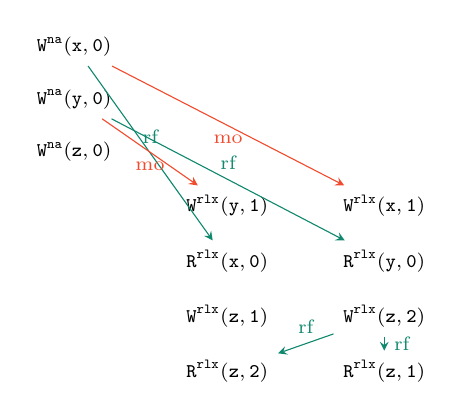
\begin{tikzpicture}[x=1pt,y=1pt,yscale=1,xscale=1]
\tikzstyle{every node}=[font=\scriptsize]
\node (initx) {$ \storeev{x}{0}{\na} $};
\node (inity) [below=5pt of initx] {$ \storeev{y}{0}{\na} $};
\node (initz) [below=5pt of inity] {$ \storeev{z}{0}{\na} $};
\node (wy1) [below right=5pt and 20pt of initz] {$ \storeev{y}{1}{\rlx} $};
\node (rx0) [below=5pt of wy1] {$ \loadev{x}{0}{\rlx} $};
\node (wz1) [below=5pt of rx0] {$ \storeev{z}{1}{\rlx} $};
\node (rz1) [below=5pt of wz1] {$ \loadev{z}{2}{\rlx} $};

\node (wx1) [right=20pt of wy1] {$ \storeev{x}{1}{\rlx} $};
\node (ry0) [below=5pt of wx1] {$ \loadev{y}{0}{\rlx} $};
\node (wz2) [below=5pt of ry0] {$ \storeev{z}{2}{\rlx} $};
\node (rz2) [below=5pt of wz2] {$ \loadev{z}{1}{\rlx} $};

\rfedge{initx}{rx0}{midway,above};
\rfedge{inity}{ry0}{midway,above};
\rfedge{wz2}{rz1}{midway,above};
\rfedge{wz2}{rz2}{midway,right};

\moedge{initx}{wx1}{midway,below};
\moedge{inity}{wy1}{midway,below};


\end{tikzpicture}
	\caption{Counter-examples in Dekker}
	\label{fig:dekker-ce}
\end{figure}

%% dekker for cppmem:
%int main() {
%	atomic_int x = 0; 
%	atomic_int y = 0;
%	atomic_int z = 0;
%	{{{ {
%					y.store(1, mo_relaxed);
%					if (x.load(mo_relaxed).readsvalue(0)) {
%						z.store(1, mo_relaxed);
%						z.load(mo_relaxed).readsvalue(1);
%					}
%				}
%				||| {
%					x.store(1, mo_relaxed);
%					if (r1=y.load(mo_relaxed).readsvalue(0)) {
%						z.store(2, mo_relaxed);
%						z.load(mo_relaxed).readsvalue(2);
%					}
%				}
%	}}};
%	return 0; 
%}



% --------------- FIG all pseudo fences -------------
\begin{figure}[!htb]
\begin{center}
\texttt{
init y := 0, x := 0;\\
	\begin{tabular}{c l || c l}
		& F$\mathtt{_{sc}}$ & & F$\mathtt{_{sc}}$\\
		(1) & W$\mathtt{_{rel}}$y(1) & (5) & W$\mathtt{_{rel}}$x(1)\\
		& F$\mathtt{_{sc}}$ & & F$\mathtt{_{sc}}$\\
		(2) & if R$\mathtt{_{rel}x}$ == 0 & (6) & if R$\mathtt{_{rel}y}$ == 0\\
		& \qquad F$\mathtt{_{sc}}$ & & \qquad F$\mathtt{_{sc}}$\\
		(3) & \qquad W$\mathtt{_{rel}}$c(1) & (7) & \qquad W$\mathtt{_{rel}}$c(0)\\
		& \qquad F$\mathtt{_{sc}}$ & & \qquad F$\mathtt{_{sc}}$\\
		(4) & \qquad assert($\mathtt{R_{rel}c}$ == 1) & (8) & \qquad assert($\mathtt{R_{rel}c}$ == 0)\\
		& \qquad F$\mathtt{_{sc}}$ & & \qquad F$\mathtt{_{sc}}$\\
	\end{tabular}
}

\divComment{All of the memory orders are rel. Is that correct?}
	\caption{Dekker's Mutual Exclusion program}\label{fig:dekker3}
\end{center}
\end{figure}

% --------- ADDING FENCES -------------
\subsection{Adding Pseudo Fences}
\par
We use a verification tool to generate a set of all the buggy traces. 
Each trace is then taken individually and analyzed. For each trace, 
the first step is inserting pseudo fences. \mosc fences are inserted 
before/after each instruction in the trace. This can be seen in 
Fig. \ref{fig:dekker3}. The fences are not actually added to the 
input program, but only added for reference purposes as a step in 
the tool. The maximum number of fences possible are added so that 
the required ones can be retained and the rest can be eliminated.

% --------------- FINDING RELATIONS -----------
\subsection{Finding relations}
% What is TO?
The C11 standard \cite{C11} states that in any valid execution 
all the \mosc instructions should form a total order. Such total order
has to be consistent with modification order and 
happens-before relation. This means that for any two \mosc instructions A 
and B such that A $ \neq B $, either $\to{\tau}{A}{B}$ or $\to{\tau}{B}{A}$. 
Hence, an execution with both $\to{\tau}{A}{B}$ and $\to{\tau}{B}{A}$ is infeasible.
% Why TO?
Our technique computes $\setSO$ of buggy execution when pseudo fences are 
present. If such $\setSO$ has a cycle, then the program with these fences 
will not have this buggy execution. 
Hence, by finding these cycles we can work out the required fences.
% Example
For example, in Fig \ref{fig:dekker2}, if the assert statement is violated
if either thread reads the value written to variable $c$ by the other thread.
% Other relations
%In order to find $\setSO$, we first compute the $\setSB$, $\setSW$, $\setHB$ and 
%$\setMO$ relations.
The basis of our approach lies upon finding relations between the 
instructions and figuring out how they affect the program in order to 
reduce the total fences to a minimum. 

\par
The next step after inserting pseudo fences is finding relations between 
instructions, including fences. 
These relations will help in figuring out which fences to eliminate from 
the trace. In particular, we are concerned with the $\setSO$ (total order) 
relations between all SC instructions and fences. Rules for TO relations 
for the C11 model are described in the official standard \cite{C11}. 
These rules are dependent relations $\setSO $, $\setSW$, $\setHB$ and $\setMO$, which 
would have to be computed first, and an order is followed for the same.

% --------------- HB -----------------
\subsubsection{Finding $\setHB$ relations}
The first and most basic relation is $\setHB$ (happens-before). 
An instruction A is said to happen-before B if:\\
($\sw{\tau}{A}{B}$) $\lor$ ($\seqb{\tau}{A}{B}$) $\lor$ ($\hb{\tau}{A}{X}$ $\land$ $\hb{\tau}{X}{B}$) $\implies$ $\hb{\tau}{A}{B}$

\par
Therefore, $\setSB$ (sequenced-before) and $\setSW$ (synchronizes-with) 
relations are computed first. 
An $\setSW$ relation is formed based on the following rules:
\begin{enumerate}
\item $\setSW$ relation between thread create and thread start instructions\\
$\sw{\tau}{thread A create}{thread A start}$

\item $\setSW$ relation between thread finish and thread join instructions\\
$\sw{\tau}{thread A finish}{thread A join}$

\item $\setSW$ relation between read (R) and write (W) instructions.\\
$\rf{\tau}{W_{\geq rel}x}{R_{\geq acq}x}$ $\implies$ $\sw{\tau}{W_{\geq rel}x}{R_{\geq acq}x}$\\
RMW operations are considered as both reads and writes in this case.
\end{enumerate}
Note that since we do not consider \moacq, \morel and \moar fences, 
our $\setSW$ rules do not capture them.
\par


% --------------- FIG --------------
%\begin{figure}
%\begin{center}
%	\makeatletter
\renewenvironment{table}%
  {\renewcommand{\familydefault}{\ttdefault}\selectfont
  \@float{table}}
  {\end@float}
\makeatother

\small
\begin{tabular}{l l l l l l l}
\hline
\textbf{\#} & \textbf{thread} & \textbf{action} & \textbf{memory order} & \textbf{location} & \textbf{value} & \textbf{rf}\\
\hline\hline
1 & 1 & thread start & seq\_cst & 0x7f012b2297e0 & 0xdeadbeef\\
\hline
2 & 1 & init atomic & relaxed & 0x60108c & 0\\
\hline
3 & 1 & init atomic & relaxed & 0x601088 & 0\\
\hline
4 & 1 & init atomic & relaxed & 0x601084 & 0\\
\hline
5 & 1 & thread create & seq\_cst & 0x7f012b329b80 & 0x7f012b329b40\\
\hline
6 & 2 & thread start & seq\_cst & 0x7f012b329be8 & 0xdeadbeef\\
\hline
7 & 2 & atomic write & relaxed & 0x601088 & 0x1\\
\hline
8 & 1 & thread create & seq\_cst & 0x7f012b329b90 & 0x7f012b329b40\\
\hline
9 & 3 & thread start & seq\_cst & 0x7f012b429ff0 & 0xdeadbeef\\
\hline
10 & 2 & atomic read & relaxed & 0x60108c & 0 & 2\\
\hline
11 & 3 & atomic write & relaxed & 0x60108c & 0x1\\
\hline
12 & 1 & thread finish & seq\_cst & 0x7f012b2297e0 & 0xdeadbeef\\
\hline
13 & 2 & atomic write & relaxed & 0x601084 & 0x1\\
\hline
14 & 3 & atomic read & relaxed & 0x601088 & 0 & 3\\
\hline
15 & 2 & atomic read & relaxed & 0x601084 & 0 & 16\\
\hline
16 & 3 & atomic write & relaxed & 0x601084 & 0\\
\hline

\end{tabular}\\

a.\\

\small
\begin{tabular}{c || c c c c c c c c c c c c c c c c c c}
\hline
instr & \textbf{0} & \textbf{1} & \textbf{2} & \textbf{3} & \textbf{4} & \textbf{5} & \textbf{6} & \textbf{7} & \textbf{8} & \textbf{9} & \textbf{10} & \textbf{11} & \textbf{12} & \textbf{13} & \textbf{14} & \textbf{15} & \textbf{16}\\
\hline\hline
0 & 0 & 0 & 0 & 0 & 0 & 0 & 0 & 0 & 0 & 0 & 0 & 0 & 0 & 0 & 0 & 0 & 0\\
\hline 
1 & 0 & 0 & 1 & 1 & 1 & 1 & 1 & 1 & 1 & 1 & 1 & 1 & 1 & 1 & 1 & 1 & 1\\
\hline 
2 & 0 & 0 & 0 & 1 & 1 & 1 & 1 & 1 & 1 & 1 & 1 & 1 & 1 & 1 & 1 & 1 & 1\\
\hline 
3 & 0 & 0 & 0 & 0 & 1 & 1 & 1 & 1 & 1 & 1 & 1 & 1 & 1 & 1 & 1 & 1 & 1\\
\hline 
4 & 0 & 0 & 0 & 0 & 0 & 1 & 1 & 1 & 1 & 1 & 1 & 1 & 1 & 1 & 1 & 1 & 1\\
\hline 
5 & 0 & 0 & 0 & 0 & 0 & 0 & 1 & 1 & 1 & 1 & 1 & 1 & 1 & 1 & 1 & 1 & 1\\
\hline 
6 & 0 & 0 & 0 & 0 & 0 & 0 & 0 & 1 & 0 & 0 & 1 & 0 & 0 & 1 & 0 & 1 & 0\\
\hline 
7 & 0 & 0 & 0 & 0 & 0 & 0 & 0 & 0 & 0 & 0 & 1 & 0 & 0 & 1 & 0 & 1 & 0\\
\hline 
8 & 0 & 0 & 0 & 0 & 0 & 0 & 0 & 0 & 0 & 1 & 0 & 1 & 1 & 0 & 1 & 0 & 1\\
\hline 
9 & 0 & 0 & 0 & 0 & 0 & 0 & 0 & 0 & 0 & 0 & 0 & 1 & 0 & 0 & 1 & 0 & 1\\
\hline 
10 & 0 & 0 & 0 & 0 & 0 & 0 & 0 & 0 & 0 & 0 & 0 & 0 & 0 & 1 & 0 & 1 & 0\\
\hline 
11 & 0 & 0 & 0 & 0 & 0 & 0 & 0 & 0 & 0 & 0 & 0 & 0 & 0 & 0 & 1 & 0 & 1\\
\hline 
12 & 0 & 0 & 0 & 0 & 0 & 0 & 0 & 0 & 0 & 0 & 0 & 0 & 0 & 0 & 0 & 0 & 0\\
\hline 
13 & 0 & 0 & 0 & 0 & 0 & 0 & 0 & 0 & 0 & 0 & 0 & 0 & 0 & 0 & 0 & 1 & 0\\
\hline 
14 & 0 & 0 & 0 & 0 & 0 & 0 & 0 & 0 & 0 & 0 & 0 & 0 & 0 & 0 & 0 & 0 & 1\\
\hline 
15 & 0 & 0 & 0 & 0 & 0 & 0 & 0 & 0 & 0 & 0 & 0 & 0 & 0 & 0 & 0 & 0 & 0\\
\hline 
16 & 0 & 0 & 0 & 0 & 0 & 0 & 0 & 0 & 0 & 0 & 0 & 0 & 0 & 0 & 0 & 0 & 0\\
\hline 
\end{tabular}

\par
\textbf{b.}\\

\normalsize
%	\caption{a. Example instruction trace from CDS Checker.\\b. Adjacency table of hb relations as formed by the tool.}
%	\label{fig:cds_hb}
%\end{center}
%\end{figure}

\par
The $\setHB$ relation is computed for all instructions before inserting the 
pseudo fences in the tool. 
This way we compute the $\setHB$ for the actual input program rather than a 
modified version of program along with pseudo fences. The advantages of this
approach are two fold. First, $\setHB$ relation is only required 
to compute the $\setMO$ (modification order) relations, which is concerned only 
with the write instructions. Therefore, computing $\setHB$ relations before 
inserting pseudo fences works as an optimization. Second, if we compute $\setHB$
after inserting fences, we will have some $\setHB$ relations that are not in 
the actual execution but will exist in the execution of program with all the 
pseudo fences. \divComment{What is the problem with having such hb?}
\divComment{Rule 1b of computing TO is also using hb, but only over write operations. So the first points still holds.}

\begin{lemma} For any valid execution of a program, the relation $\setHB$ computed 
	as above is same as \emph{happens-before} of C11.
\end{lemma}

% --------------- MO ------------
\subsubsection{Finding $\setMO$ relations}
$\setMO$ relations are formed between write instructions when the value of a 
variable is changed at some point in the program. The rules for modification 
order as described by the standard \cite{C11} are:
\begin{enumerate}
    \item Write-write coherence: \\
    $\hb{\tau}{A_x}{B_x}$ $\implies$ $\mo{\tau}{A_x}{B_x}$\\
    \textit{where A, B are write operations modifying variable x}
    
    \item Read-read coherence:\\
    $\hb{\tau}{\rf{\tau}{X_x}{A_x}}{B_x}$ $\implies$ ($\rf{\tau}{X_x}{B_x}$) $\lor$\ ($\rf{\tau}{\mo{\tau}{X_x}{Y_x}}{B_x}$)\\
    \textit{where X, Y are writes on x\\ and A, B are reads on x}
    
    \item Read-write coherence:\\
    $\hb{\tau}{A_x}{B_x}$ $\implies$ ($\rf{\tau}{X_x}{A_x}$) $\land$\ ($\mo{\tau}{X_x}{B_x}$)\\
    \textit{where X, B are writes on variable x\\and A is a read on variable x}
    
    \item Write-read coherence:\\
    $\hb{\tau}{X_x}{B_x}$ $\implies$ ($\rf{\tau}{X_x}{B_x}$) $\lor$\ ($\rf{\tau}{\mo{\tau}{X_x}{Y_x}}{B_x}$)\\
    \textit{where X, Y are writes on variable x\\and B is a read on variable x}
\end{enumerate}

\begin{lemma}
	For any valid execution of a program, the relation $\setMO$ computed 
	as above is same as \emph{modification-order} of C11.
\end{lemma}

\par
After this step, the pseudo fences are inserted.

% --------------- TO -----------
\subsubsection{Finding $\setSO$ relations between SC instructions}\label{to_rel}
The final step in finding relations and the main step that is required for 
fence elimination is to find $\setSO$ relations. The rules for $\setSO$ relations 
in the C11 standard are defined in \cite{C11}. These rules can be interpreted 
as the following:
%\tikzset{
    %Define standard arrow tip
    >=stealth',
    %Define style for boxes
    punkt/.style={
           rectangle,
           minimum height=2em,
           text centered},
}

\begin{enumerate}
\setcounter{enumi}{-1}
\item
	For a given variable, if there is a read from relation between a read and a write instruction, then the SC instructions above the write are in TO with the SC instructions below the read.\\
	\begin{tikzpicture}[baseline = (current bounding box.north)]
    \node[punkt] (x) {X:$F_{sc}$};
    \node[punkt,below=of x] (a) {A:$Wx$}
        edge[-](x);
    \node[punkt,right=of x] (b) {B:$Rx$};
    \node[punkt, below=of b] (y) {Y:$F_{sc}$}
    	edge[-](b);
  	\draw [->] (a) -> (b) node[midway,above] {rf};
    \end{tikzpicture}\\
    \rf{A}{B} $\implies$ \too{X}{Y}

\item
	\begin{enumerate}[a.]
	\item
		For a given variable, for an SC read instruction reading from an SC write instruction, there is a TO relation between the read and the write instructions.\\
		\rf{A:$W_{sc}$}{B:$R_{sc}$}\\
		\too{A}{B}
	
	\item
		For a given variable,, for an SC read instruction reading from a write instruction \textit{M}, the read instruction is in TO with all SC write instruction which happen after \textit{M}.\\
		A:$W_{sc}x$, M:$Wx$, B:$R_{sc}x$\\
		\hb{M}{A} $\land$ \rf{M}{B} $\implies$ \too{B}{A}
	\end{enumerate}

\item
	For a given variable, all SC instructions above a read instruction reading from a write instruction \textit{$M_1$} are in TO with all SC write instruction modifying the variable after \textit{$M_1$}.
	\begin{tikzpicture}[baseline = (current bounding box.north)]
	\node[punkt](x) {X:$F_{sc}$};
	\node[punkt, below=of x](b) {B:$Rx$}
		edge[-](x);
	\node[punkt, right=of b](m1) {M$_1:Wx$};
	\node[punkt, below=of m1](m2) {M$_2:W_{sc}$};
  	\draw [->] (m1) -> (b) node[midway,above] {rf};
  	\draw [->] (m1) -> (m2) node[midway,right] {mo};
  	\end{tikzpicture}\\
  	\too{X}{M$_2$}
 
\item
	\begin{tikzpicture}[baseline = (current bounding box.north)]
	\node[punkt](a) {A:$Wx$};
	\node[punkt, below=of a](x) {X:$F_{sc}$}
		edge[-](a);
	\node[punkt, right=of a](y) {Y:$F_{sc}$};
	\node[punkt, below=of y](b) {B:$Rx$}
		edge[-](y);
	\node[punkt, right=of y](m) {M:$Wx$};
	\end{tikzpicture}\\
	\rf{M}{B} $\land$ \mo{M}{A} $\implies$ \too{Y}{X}

\item
	\begin{tikzpicture}[baseline = (current bounding box.north)]
	\node[punkt](a) {A:$Wx$};
	\node[punkt, below=of a](x) {X:$F_{sc}$}
		edge[-](a);
	\node[punkt, right=of a](y) {Y:$F_{sc}$};
	\node[punkt, below=of y](b) {B:$Wx$}
		edge[-](y);
	\end{tikzpicture}\\
	\begin{enumerate}[a.]
	\item if B:$W_{sc}x$\\
		\mo{B}{A} $\implies$ \too{B}{X}
	
	\item if A:$W_{sc}x$\\
		\mo{B}{A} $\implies$ \too{Y}{A}
	
	\item
		\mo{B}{A} $\implies$ \too{Y}{X}
	\end{enumerate}
	
\end{enumerate}
\textit{Note: ``the fence above instruction A'' is a comprehensive term for all 
	the fences which are sequenced-before instruction A.}
Intuitively, transitive closure of $\setSO$ is \emph{sc} ordering over the 
given program execution if the program had the pseudo fences to begin with.
Such an execution may or may not be valid under C11 memory model.

\begin{theorem}
	For any valid execution of a program, the transitive closure of $\setSO$ 
	is the same as \emph{to} order of C11 of in the corresponding (possibly 
	invalid) trace with candidate fences.
\end{theorem}


% --------------- SOLN EXPLAINED -------------
\subsection{Eliminating Fences}
The rules in \textsection\ref{to_rel} provides us $\setSO$ relations between all 
instructions and fences. We now get a graph that would look 
like Fig \ref{fig:cycles}. 

%Further, the transitivity of $\setSO$ 
%relation will give us some additional pair in $\setSO$. 

\par
The purpose of creating a graph this way is to detect if there are any cycles 
formed in the trace after inserting the fences. 
In a total order 
%relation, the antisymmetry and connexity properties state that:\\
%Either \too{A}{B} or \too{B}{A} and if (\too{A}{B} $\land$ \too{B}{A}) then A = B.\\
%This property of TO can be exploited to minimize the fences. 
According to the C/C++11 standard, each \mosc instruction is in total order 
with every other \mosc instruction. This means that for any two \mosc 
instructions A and B, either $\to{\tau}{A}{B}$ or $\to{\tau}{B}{A}$. According to 
$\setSO$ rules, if both of these relations hold true, then A = B. 
If A $\neq$ B and A and B are different entities which satisfy the 
relation ($\to{\tau}{A}{B}$ $\land$ $\to{\tau}{B}{A}$), that means that a cycle is 
formed between instructions A and B. This, in turn, violates the $\setSO$ 
property, rendering the execution infeasible. If a certain execution 
becomes infeasible, then it would never exhibit during an actual execution 
of the program.

Note that apart from the rules described above, some $\setSO$ edges 
will be created due to the transitivity of $\setSO$.
We have not included these edges in our final graph and limited 
the edges in graphs to the set that was computed using the rules 
in \textsection\ref{to_rel}. That is, all $\setSB$ edges are taken into 
consideration whether immediate 
or not, and only those edges formed via the $\setSO$ rules discussed in 
section \textsection\ref{to_rel} are considered while forming a graph. 
The reason of this is explained in \textsection\ref{sec:no-transitive}.


% --------------- FIG 5 -------------------
\begin{figure}
\begin{center}
	\tikzset{
    %Define standard arrow tip
    >=stealth',
    %Define style for boxes
    punkt/.style={
           rectangle,
           minimum height=2em,
           text centered},
}

\begin{tikzpicture}
    \node[punkt] (f1n1) {$F_1n_1$};
    \node[punkt,below=of f1n1] (f1n2) {$F_1n_2$}
        edge[<-](f1n1);
    \node[punkt,below=of f1n2] (f1n3) {$F_1n_3$}
        edge[<-](f1n2);
    \node[punkt,below=of f1n3] (f1n4) {$F_1n_4$}
        edge[<-](f1n3);
    \node[punkt,right=of f1n1] (f2n1) {$F_2n_1$};
    \node[punkt,below=of f2n1] (f2n2) {$F_2n_2$}
        edge[<-](f2n1)
        edge[<-](f1n2);
    \node[punkt,below=of f2n2] (f2n3) {$F_2n_3$}
        edge[<-](f2n2)
        edge[->](f1n2);
    \node[punkt,right=of f2n1] (f3n1) {$F_3n_1$};
    \node[punkt,below=of f3n1] (f3n2) {$F_3n_2$}
        edge[<-](f3n1)
        edge[->,bend left=25](f2n2)
        edge[<-,bend right=25](f2n2)
        edge[->,bend right=45](f1n1);
    \node[punkt,below=of f3n2] (f3n3) {$F_3n_3$}
        edge[<-](f3n2);
    \node[punkt,below=of f3n3] (f3n4) {$F_3n_4$}
        edge[<-](f3n3);
    
\end{tikzpicture}\\
	\caption{A graph structure created by various relations acting as edges}
	\label{fig:cycles}
\end{center}
\end{figure}

\subsection{Restricting Buggy Executions}
\par
We find out $\setSO$ relations in only the buggy or erroneous traces which 
are obtain from verification tool. For each erroneous trace, a graph is 
formed with the instructions/fences as nodes and the $\setSO$ relations as 
edges. 
Our purpose is to insert fences such that the graph of the buggy exection 
will contain a cycle 
When such a cycle is introduced, it violates the properties of a total 
order relation in C11, rendering the entire execution infeasible. 
An infeasible execution will never occur during runtime, which means 
that the buggy execution in which the $\setSO$ cycle is introduces using 
fences will never be executed. 
Hence the assertion which was being violated will remain satisfied. 

In case there are no cycles forming for one or more of the buggy traces, 
the behavior is deemed to be unpreventable using \mosc fences. 

\par
In Fig \ref{fig:cycles}, a number of cycles can be noted. Some of them are:
\begin{itemize}
\item \textit{$I_1n_1 \rightarrow F_2n_2 \rightarrow I_2n_1 \rightarrow I_1n_1$}
\item \textit{$F_2n_2 \rightarrow F_3n_2 \rightarrow F_2n_2$}
\item \textit{$F_1n_1 \rightarrow I_1n_1 \rightarrow F_2n_2 \rightarrow F_3n_2 \rightarrow F_1n_1$}
\item \textit{$I_1n_1 \rightarrow F_2n_2 \rightarrow F_3n_2 \rightarrow F_2n_2 \rightarrow I_2n_1 \rightarrow I_1n_1$}
\end{itemize} 
A single cycle out of the above mentioned or others being formed needs 
to be created in order to prevent this particular run from ever taking 
place. From just looking over it once, one can notice that the smallest 
cycle would be \textit{$F_2n_2 \rightarrow F_3n_2 \rightarrow F_2n_2$} 
with just two participating nodes. However, the cycle with the least 
number of fences is \textit{$I_1n_1 \rightarrow F_2n_2 \rightarrow I_2n_1 
\rightarrow I_1n_1$} with just one fence (\textit{$F_2n_2$}) being inserted. 
Hence, if just \textit{$F_2n_2$} is inserted into the program, this particular 
buggy trace will be stopped. This method is carried out for all such 
buggy traces and their cycles are calculated and stored.

Another point to note is that, for each cycle, only the fences are considered
while calculating the final result. This is because the instructions present in the
cycles (if any) are already present in the input program and are immutable.
The fences, on the other hand, are the inserted by us and therefore are the only
entities considered while finding the final result.


\begin{lemma}
	Introducing fences in any cycle of $\setSO$ will stop that cycle 
	from forming in actual run of the program.
\end{lemma}

\begin{lemma}
	If there are no cycles in $\setSO$ of a buggy execution, the behavior 
	cannot be stopped using any C11 fences.
\end{lemma}

\begin{theorem}
	Stopping all cycles of $\setSO$ in any buggy execution will stop that
	buggy execution in actual run of program.
\end{theorem}

% --------------- FENCE MIN PROBLEM ----------
\subsection{The Fence Minimization Problem} \label{sec:fence-min}
\par
Even if cycles are calculated for each trace, the solution for obtaining 
a minimized number of fences to be inserted is not so straight-forward 
as simply choosing the one with the minimum fences for each trace. 
For one, there might be multiple cycles containing minimum fences. 
Another issue is that this would not yield the actual minimized 
number of fences. 

% --------------- FIG 6 -------------------
\begin{figure}
\begin{center}
	Cycles from trace 1:\\
	\textit{$F_1 \rightarrow F_2 \rightarrow I_1 \rightarrow F_1$}\\
	\textit{$F_3 \rightarrow F_4 \rightarrow F_1 \rightarrow F_3$}\\
	Cycles from trace 2:\\
	\textit{$F_3 \rightarrow F_4 \rightarrow F_3$}
	\caption{Example cycles from traces}
	\label{fig:fence_min}
\end{center}
\end{figure}

Fig \ref{fig:fence_min} shows cycles from two buggy traces from 
a program. 
one solution to obtain the minimum number of fences was 
to take the smallest cycle from each trace, that is to take the 
cycle which contains the least number of fences from each execution 
trace. In this case, fences \textit{$F_1$}, \textit{$F_2$} 
would be chosen from trace 1 and fences \textit{$F_3$}, \textit{$F_4$} 
would be chosen from trace 2. This makes four total fences that 
to include in the main program to stop the behavior where 
any assertion gets violated.

\par
However, this is not the optimal solution. Fig \ref{fig:fence_form} 
shows the example explained in Fig \ref{fig:fence_min} converted 
into its respective formula in propositional logic. For each trace, 
the cycles are added as disjunctions, with each fence in a cycle 
being a necessary component, deeming it a conjunction. Since each 
trace needs to satisfy at least one cycle for the trace to become 
infeasible, each cycle is a disjunction. All traces need to be 
prevented, so each trace is part of a conjunction. Let 
$ \mathcal{B} $ be the set of all buggy execution of a program with 
at least one cycle. Let $ \mathcal{F}(\mathcal{B}) $ gives the 
fence minimization formula for set of buggy executions $ \mathcal{B} $.

% --------------- FIG 7 -----------------
\begin{figure}
\begin{center}
	( ( $F_1 \land F_2\ ) \lor\ ( F_3 \land F_4 \land F_1\ )\ ) \land\ (\ (\ F_3 \land F_4$ ) )
	\caption{Formula for Fig \ref{fig:fence_min}}
	\label{fig:fence_form}
\end{center}
\end{figure}

\par
The formula in fig \ref{fig:fence_form} can be looked at as a 
cost function to minimize the cost, with each entity being a fence, 
having value either 0 or 1. A fence having value 1 would mean that 
it should be inserted in the program and value 0 would mean that 
it should not be inserted in the program, according to the 
minimized cost. From this formula, the solution for Fig \ref{fig:fence_min} 
comes out to have 3 fences – \textit{$F_3, F_4, F_1$}, 
unlike the original solution where four fences were sought.

\begin{theorem}
	For any input program $ \mathcal{F}(\mathcal{B}) $ gives optimal
	number of fences required to stop all the buggy behaviors in 
	$ \mathcal{B} $.
\end{theorem}

\par
Implementing such a propostional formula for programs with 
more than 50 execution traces, with each of them having uncountable 
fences would be quite an overhead. An SMT/SAT Solver is used for 
this purpose. Our tool uses Z3 to find minimum satisfying assignment 
of such formulas. A formula similar to the one in Fig \ref{fig:fence_form} 
is created for each program and the minimum cost with the maximum 
satisfying assignment is computed. 

\begin{algorithm}
\caption{Our algorithm}
\begin{algorithmic}[1]

\Procedure{}{input\_file}
    \State traces = model\_checker(input\_file)
    \For{each trace}
    	\State hb = find\_hb()
		\State mo = find\_mo(hb)
		\State updated\_trace = add\_pseudo\_fences()
		\State sb = find\_sb(updated\_trace)
		\State to = find\_to(updated\_trace)
%		\State to += sb
		\State cycles = find\_cycles()
    	\If{cycles} \Comment{if cycles are formed}
        	\State z3\_variables = find\_fence\_locations()
	        \State translate\_cycles\_to\_z3(z3\_variables)
        \Else
    	    \State ``This behaviour cannot be stopped using SC fences''
			\State exit()
        \EndIf
    \EndFor
    
    \State create\_z3\_file()
	\State fences\_required = run\_z3\_file()
	\State insert\_into\_input\_file(fences\_required)
\EndProcedure

\end{algorithmic}
\end{algorithm}


\subsubsection{why transitive TO edges aren't considered} \label{sec:no-transitive}
The relations which are considered to form the final graph are - 
all $\setSB$ edges between only \mosc instructions including transitive $\setSB$ edges, 
and directly formed $\setSO$ edges but not transitively formed $\setSO$ edges.  
This is because transitively formed $\setSO$ relations will be of 
no use in our case. If there is a transitive $\setSO$ relation formed 
between two instructions, then this relation has been caused by 
some other edges in our graph. 
Our formula is concerned only with the cycles in the graph 
(as discussed in \textsection\ref{sec:fence-min}), we will focus on 
the new cycles that might come if we were to consider the transitive 
edges. These cycles might be formed because of two reasons - 
either the new cycle consists of i) some transitive edges in the 
actual program that we did not include in $\setSO$, or ii) some 
transitive edges created due to pseudo fences. In case i), the cycle 
(let $C$) is certainly caused by some pseudo fence inserted in the program 
since the actual program execution cannot have a cycle. Since the 
transitive edge is formed due to some edge in our $\setSO$, there 
will be a representative cycle $C'$ of the cycle $C$ formed using 
edges in $\setSO$. As our formula only concerns the pseudo fences, 
the formula constructed for $C$ and $C'$ will be the same. 
Similarly in case ii), since the cycle is created due to transitive 
edge caused by one or more fences, the formula must consist these 
fences too as a way to determine which fences caused the cycle. Hence,
the formula remains same. 

%Even if we were to consider these edges, the formula will not change. 
%Therefore, for this transitive 
%relation, we need not consider the two nodes participating in the 
%transitive edge, instead we need to consider the original nodes 
%which caused this transitive relation to form in the first place. 
%Transitive edges are formed through transitive relations which will 
%hide the originally formed TO relations. But by excluding the 
%original edges, the transitive edges we need will never actually be formed.

For instance, look at Fig \ref{fig:cycles}. The edge \textit{$F_3n_2$} 
$\rightarrow$ \textit{$I_1n_1$} is not an edge found through the rules of 
TO relations. It is a transitive edge. So if we were to consider the cycle 
\textit{$F_3n_2$} $\rightarrow$ \textit{$I_1n_1$} $\rightarrow$ \textit{$F_2n_2$}
$\rightarrow$ \textit{$F_3n_2$}, we notice that the edge \textit{$F_3n_2$} 
$\rightarrow$ \textit{$I_1n_1$} cannot exist on its own. Hence we cannot simply 
consider the three edges which partake in the formation of this cycle.
We will need to consider all the possible edges which caused the formation of the 
transitive edge, which are:
\begin{enumerate}
	\item \textit{$F_3n_2$} $\rightarrow$ \textit{$F_2n_2$} $\rightarrow$ 
\textit{$I_2n_1$} $\rightarrow$ \textit{$I_1n_1$}
	\item \textit{$F_3n_2$} $\rightarrow$ \textit{$F_1n_1$} $\rightarrow$ \textit{$I_1n_1$}
\end{enumerate}

Hence the cycle \textit{$F_3n_2$} $\rightarrow$ \textit{$I_1n_1$} $\rightarrow$
\textit{$F_2n_2$} $\rightarrow$ \textit{$F_3n_2$} translates into the following cycles:
\begin{enumerate}
	\item \textit{$F_3n_2$} $\rightarrow$ \textit{$F_2n_2$} $\rightarrow$ \textit{$I_2n_1$} 
$\rightarrow$ \textit{$I_1n_1$} $\rightarrow$ \textit{$F_2n_2$} $\rightarrow$ \textit{$F_3n_2$}
	\item \textit{$F_3n_2$} $\rightarrow$ \textit{$F_1n_1$} $\rightarrow$ \textit{$I_1n_1$} $\rightarrow$
\textit{$F_2n_2$} $\rightarrow$ \textit{$F_3n_2$}
\end{enumerate}


\par
So even if transitive $\setSO$ relations are considered as graph edges, 
they would not impact our final solution. 
%For each transitively 
%formed edge, all original edges which would have possibly caused 
%the transitive edge would be needed to be kept track of. 
Therefore, using just the original edges serves our purpose 
in a much more efficient manner.

\section{Implementation Details} \label{sec:implementation}
\ourtechnique attempts to invalidate a buggy trace 
by inserting \cc fences in the input program $P$
by the technique discussed in Sections
\ref{sec:invalidating ce} and \ref{sec:methodology}.
%
The technique relies on a {\em counter example generator} 
to provide buggy traces (or counter examples) containing
the $\setMO$, $\setHB$ and $\setRF$ relations between the 
events of each buggy trace (line 3, 
Algorithm~\ref{alg:main algo}).
%
We recognized \cds \cite{cds} as the closest match to the
specification of a counter example generator
for the following reasons;

\begin{enumerate}
	\item \cds is a stateless model checker that returns traces 
		with assert violations (or buggy traces) if any.
	
	\item Unlike competing alternatives, \cds does not halt at the detection 
		of the first buggy trace instead it continues to provide all buggy 
		traces as required by \ourtechnique.
	
	\item \cds also provides $\setRF$ and $\setSB$ relations between the events 
		of the buggy trace. The information returned by \cds is sufficient
		to compute the $\setHB$ and $\setMO$ relations.
	
	\item Competing alternatives that return buggy traces for an input
		program, namely \genmc \cite{genmc-PLDI19} and \tracer \cite{tracer2018}, 
		do not support our requirements.
		%
		\genmc is designed for a variant of \cc \cite{LahavVafeiadis-PLDI17} and
		does not support an option for returning all buggy traces. \tracer is
		designed for a subset of \cc that has no support for \sc, \na or \rel 
		memory orders. \snj{What about Herd?}
\end{enumerate}

To bridge the gap between \cds's output and \ourtechnique's requirement,
we perform a pre-processing step that uses the $\setSB$ and $\setRF$ relations 
provided by \cds to compute the $\setHB$ and $\setMO$ relations on the events
of the buggy traces, based on the coherence rules provided by \cc model.
%
The buggy traces along with $\setSB$, $\setRF$ and computed $\setHB$ 
and $\setMO$ relations are provided as input to the core technique 
(lines 4-14, Algorithm~\ref{alg:main algo}) for synthesizing fences as
discussed in Section~\ref{sec:methodology}.

The core technique and the pre-processing has been implemented in 
{\tt Python}.
\ourtechnique uses {\em Johnson's} algorithm provided in {\em networkx}
library to detect cycles in \hlref{coherence conditions} and
\sc total order over 
events of the intermediate trace that includes the 
candidate fences (lines 7-8, Algorithm~\ref{alg:main algo}).
%
Upon finding cycles, \ourtechnique generates a SAT query 
representing the non-optimal set of candidate fences and
uses \z theorem prover to find the {\em min-model} of the 
query (line 11,13, Algorithm~\ref{alg:main algo}).

\noindent
{\bf Time efficient alternative technique:} It was observed that analysis
time of the core technique and \z computation of min-model were impacted
by the number of buggy traces returned by \cds.
%
As a counter measure we propose a time efficient alternative to the core 
technique that considers one buggy trace at a time.
%
This technique picks any one buggy trace of input program $P$,
fixes the same by inserting fences and  transforms $P$ to $P'$,
where $P'$ contains the newly added fences along with the events 
originally in $P$. 
%
The technique then looks for the next buggy trace by invoking \cds 
with $P'$ as the input program. 
The process repeats till \cds returns no buggy traces, or
finds a buggy trace that cannot be fixed with \cc fences.

\begin{wrapfigure}{l}{0.45\textwidth}
	\vspace{-2.5em}
	\begin{tabular}{|l|}
		\multicolumn{1}{r}{\scriptsize $e_i$: program events,
			$\mathbb{F}_i$: candidate fences} \\
		
		\hline
		cycles in $\tau_1$ (${\tt C}_{\tau_1}$)\\
		\tab $\mathbb{F}_1$ $R$ $\mathbb{F}_2$ $R$ $e_1$ $R$ $\mathbb{F}_1$\\
		\tab $\mathbb{F}_3$ $R$ $\mathbb{F}_4$ $R$ $\mathbb{F}_1$ $R$ $\mathbb{F}_3$\\
		$\formula{{\tt C}_{\tau_1}}$ = ($\mathbb{F}_1 \^ \mathbb{F}_2$) $\v$ ($\mathbb{F}_1 \^ \mathbb{F}_3 \^ \mathbb{F}_4$)\\
		\\
		cycles in $\tau_2$ (${\tt C}_{\tau_2}$)\\
		\tab $\mathbb{F}_3$ $R$ $\mathbb{F}_4$ $R$ $\mathbb{F}_3$\\
		$\formula{{\tt C}_{\tau_2}}$ = ($\mathbb{F}_3 \^ \mathbb{F}_4$)\\
		\hline
				
		\multicolumn{1}{c}{\footnotesize\hl{3-fence}}
	\end{tabular}
	\vspace{-3em}
\end{wrapfigure}

The technique is sound, \ie if the buggy traces can be stopped by 
inserting \cc fences in the program then the technique will successfully
invalidate those traces;
but the technique is not optimal in the number of fences inserted.
The non-optimality of the efficient version is a result of the reduction
in information that the technique has to work with (from all buggy traces
to just one at a time). As a consequence of considering one trace per
iteration the \z formula is attenuated with terms only from one trace.
%
Consider the example in Figure~\hlref{3-fence} 
depicting cycles in two buggy traces $\tau_1$ and $\tau_2$ of an 
input program. The primary \ourtechnique 
technique would provide the formula $\formula{{\tt C}_{\tau_2}}$ $\^$ 
$\formula{{\tt C}_{\tau_2}}$ to \z and thus recognize ($\mathbb{F}_1 \^ 
\mathbb{F}_3 \^ \mathbb{F}_4$) as the optimal solution.
The time efficient version, however, may consider the formula 
$\formula{{\tt C}_{\tau_1}}$ in the first iteration and 
$\formula{{\tt C}_{\tau_2}}$ in the next iteration and return
($\mathbb{F}_1 \^ \mathbb{F}_2$) $\^$ ($\mathbb{F}_3 \^ \mathbb{F}_4$) 
as the result which is not optimal in the number of fences.

However, it was observed from the experimental results that the time
efficient technique significantly outperforms the primary technique in terms of 
the analysis time while adding a reasonably small number of extra
fences. The experimental results have been discussed in the 
following section.

\section{Results} \label{sec:results}
\begin{table}
		\resizebox{\columnwidth}{!}{%
\begin{tabular}{l|r|r|r|r|r|r|r|l}
\multicolumn{1}{c|}{}                       & \multicolumn{1}{c|}{}                                                                             & \multicolumn{1}{c|}{}                                                                            & \multicolumn{1}{c|}{}                                                                                                & \multicolumn{4}{c|}{\textit{Times (in seconds)}}                                                                        & \multicolumn{1}{c}{}                                    \\ \cline{5-8}
\multicolumn{1}{c|}{\multirow{-2}{*}{Name}} & \multicolumn{1}{c|}{\multirow{-2}{*}{\begin{tabular}[c]{@{}c@{}}Buggy\\ executions\end{tabular}}} & \multicolumn{1}{c|}{\multirow{-2}{*}{\begin{tabular}[c]{@{}c@{}}Fences\\ inserted\end{tabular}}} & \multicolumn{1}{c|}{\multirow{-2}{*}{\begin{tabular}[c]{@{}c@{}}Avg no. of\\ instr/trace\end{tabular}}} & \multicolumn{1}{c|}{\cite{cds}} & \multicolumn{1}{c|}{\z} & \multicolumn{1}{c|}{Tool only} & \multicolumn{1}{c|}{Total} & \multicolumn{1}{c}{\multirow{-2}{*}} \\ \hline
dekker\_no\_fence                           & 2                                                                                                 & 2                                                                                                & 19                                                                                                                   & 0.30                            & 0.02                    & {\color[HTML]{00009B} 0.02}    & 0.34                       \\
fib\_mod\_false-unreach-call                & 12                                                                                                & 3                                                                                                & 32                                                                                                                   & 4.44                            & 0.36                    & {\color[HTML]{00009B} 1.93}    & 6.74                       \\
mot\_eg\_modified                           & 292                                                                                               & 4                                                                                                & 40                                                                                                                   & 0.73                            & 0.12                    & {\color[HTML]{00009B} 3.99}    & 4.83                       \\
mot\_eg\_v2\_2                              & 1835                                                                                              & 2                                                                                                & 32                                                                                                                   & 2.56                            & 0.03                    & {\color[HTML]{00009B} 12.18}   & 14.77                      \\
mot\_eg\_v3                                 & 19                                                                                                & 2                                                                                                & 26                                                                                                                   & 0.26                            & 0.02                    & {\color[HTML]{00009B} 0.10}    & 0.37                       \\
mot\_eg\_v3\_modified                       & 29                                                                                                & 5                                                                                                & 27                                                                                                                   & 0.25                            & 0.02                    & {\color[HTML]{00009B} 0.14}    & 0.41                       \\
peterson                                    & 24                                                                                                & 2                                                                                                & 24                                                                                                                   & 0.28                            & 0.03                    & {\color[HTML]{00009B} 0.67}    & 0.98                       \\
read\_write\_lock\_2                        & 524                                                                                               & 4                                                                                                & 41                                                                                                                   & 1.42                            & 6.60                    & {\color[HTML]{00009B} 84.69}   & 92.70                      \\
read\_write\_lock\_unreach\_11              & 1                                                                                                 & 2                                                                                                & 27                                                                                                                   & 0.24                            & 0.02                    & {\color[HTML]{00009B} 0.02}    & 0.28                       \\
read\_write\_lock\_unreach\_12              & 58                                                                                                & 2                                                                                                & 34                                                                                                                   & 0.43                            & 0.02                    & {\color[HTML]{00009B} 0.55}    & 0.99                       \\
read\_write\_lock\_unreach\_13              & 9229                                                                                              & 2                                                                                                & 44                                                                                                                   & 55.51                           & 0.09                    & {\color[HTML]{00009B} 153.14}  & 208.74                     \\
basic                                       & 1                                                                                                 & 2                                                                                                & 21                                                                                                                   & 0.33                            & 0.01                    & {\color[HTML]{00009B} 0.01}    & 0.35                       &                                                         \\
mixed\_eg                                   & 4                                                                                                 & 4                                                                                                & 27                                                                                                                   & 0.33                            & 0.02                    & {\color[HTML]{00009B} 0.06}    & 0.41                       &                                                         \\
dekker\_rlx                                 & 2                                                                                                 & 2                                                                                                & 17                                                                                                                   & 0.32                            & 0.01                    & {\color[HTML]{00009B} 0.35}    & 0.01                       														\\
pgsql0                                      & 7                                                                                                 & 2                                                                                                & 23                                                                                                                   & 0.27                            & 107.13                  & {\color[HTML]{00009B} 603.75}  & 496.35                     \\
publish-sc0                                 & 41                                                                                                & 3                                                                                                & 55                                                                                                                   & 0.36                            & 0.01                    & {\color[HTML]{00009B} 4.60}    & 4.24                       \\
publish-sc1                                 & 41                                                                                                & 3                                                                                                & 55                                                                                                                   & 0.30                            & 0.01                    & {\color[HTML]{00009B} 4.56}    & 4.25                       \\
SB+assert0                                  & 1                                                                                                 & 2                                                                                                & 15                                                                                                                   & 0.32                            & 0.01                    & {\color[HTML]{00009B} 0.34}    & 0.01                       \\
SB+assert1                                  & 1                                                                                                 & 2                                                                                                & 15                                                                                                                   & 0.32                            & 0.01                    & {\color[HTML]{00009B} 0.34}    & 0.01                       \\
thread01                                    & 2                                                                                                 & 2                                                                                                & 13                                                                                                                   & 0.32                            & 0.02                    & {\color[HTML]{00009B} 0.35}    & 0.01                       \\
2+2W0053                                    & 1                                                                                                 & 2                                                                                                & 22                                                                                                                   & 0.33                            & 0.02                    & {\color[HTML]{00009B} 0.36}    & 0.02                       \\
2+2W                                        & 1                                                                                                 & 2                                                                                                & 18                                                                                                                   & 0.32                            & 0.01                    & {\color[HTML]{00009B} 0.35}    & 0.01                       \\
3.2W+lwsync+lwsync+po                       & 1                                                                                                 & 3                                                                                                & 28                                                                                                                   & 0.33                            & 0.02                    & {\color[HTML]{00009B} 0.37}    & 0.02                       \\
DETOUR0928                                  & 1                                                                                                 & 2                                                                                                & 29                                                                                                                   & 0.33                            & 0.02                    & {\color[HTML]{00009B} 0.37}    & 0.02                       \\
m2                                          & 9                                                                                                 & 2                                                                                                & 28                                                                                                                   & 0.33                            & 0.01                    & {\color[HTML]{00009B} 0.47}    & 0.12                       \\
mc                                          & 3                                                                                                 & 2                                                                                                & 39                                                                                                                   & 0.34                            & 0.01                    & {\color[HTML]{00009B} 0.46}    & 0.10                       \\
MOREDETOUR0398                              & 4                                                                                                 & 2                                                                                                & 43                                                                                                                   & 0.45                            & 0.02                    & {\color[HTML]{00009B} 0.64}    & 0.18                       \\
MOREDETOUR0406                              & 3                                                                                                 & 2                                                                                                & 47                                                                                                                   & 0.55                            & 0.02                    & {\color[HTML]{00009B} 0.74}    & 0.17                       \\
MOREDETOUR0685                              & 5                                                                                                 & 2                                                                                                & 48                                                                                                                   & 0.93                            & 0.02                    & {\color[HTML]{00009B} 1.28}    & 0.33                       \\
MOREDETOUR0687                              & 1                                                                                                 & 2                                                                                                & 36                                                                                                                   & 0.34                            & 0.02                    & {\color[HTML]{00009B} 0.40}    & 0.04                       \\
MOREDETOUR0874                              & 2                                                                                                 & 2                                                                                                & 38                                                                                                                   & 0.36                            & 0.03                    & {\color[HTML]{00009B} 0.48}    & 0.10                                                         
\end{tabular}%
}
	\caption{Bare bone results}
	\label{tab:results1}
\end{table}

In order to analyze and evaluate the performance of the algorithm 
proposed in this paper, we created a tool called ----. 77 benchmarks were
executed on it, using a computer with \ishComment{specs}.
Most of these benchmarks have been acquired from verification tool
repositories, namely CDSChecker \cite{cds}, Tracer \cite{tracer2018},
GenMC \cite{genmc-PLDI19}, RCMC \cite{rcmc-POPL18}, Watts \cite{watts}.
These benchmarks have been modified in terms of format to replicate the
one required by CDSChecker's input programs.
Some programs were translated into C11 and suitable
memory orders were added where no memory orders were specified.

All benchmarks can be segregated into two base classes. The first set consists of 
programs whose buggy executions can be stopped by inserting fences. Table \ref{tab:results1}
summarizes these results. The second category of benchmarks contains programs which
either do not provide obtainable results using a model checking tool, or
whose buggy behaviours cannot be stopped simply by using fences. \textit{\{The reason
for this may be because those programs are semantically created to prove
a point instead of being stopped using fences.\}} Benchmarks range from
having a few buggy executions to having thousands of buggy executions. They
also vary in the number of threads and atomic instructions in each of
their traces.

For each concurrent program, we provide the following information as criteria for evaluation:
the number of buggy executions found by the model checker, the number of fences
inserted in the final program, and the average number of atomic instructions
in each trace. The tool is assessed by being timed according to different steps
of the program, including time taken by the model checker, time taken by the
SAT solver and the computation time taken by the tool itself. Programs
were run in two modes- the regular mode with all executions
being taken into account and the \texttt{-t} flag mode, where only the first
trace was taken into consideration for each iteration of the input program.

\begin{figure}
	a. $O(n^3)$, \\
	\textit{where n is the number of vertices}
	
	
	b. $O((n+e)(c+1))$, \\
	\textit{for n nodes, e edges and c elementary circuits}
	\caption{a. complexity of computing transitive \lhb relations\\
	b. complexity of Johnson's algorithm to compute all elementary cycles in a graph}
\end{figure}

Through experiments, it was also observed that the two most expensive 
operations in the entire process were computing transitive relations for \lhb
relations, and computing all possible elementary cycles in the graph of \lto
relations. The metric, ``number of instructions in each trace'' adds
considerably to the former factor. A large number of instructions in each
trace produces a greater number of \lhb relations, thereby resulting in
greater computation time for transitive relations. This is evidenced by the benchmarks
\texttt{publish-sc0} and \texttt{publish-sc1} where the number of instructions in each
execution trace is 55 - a greater than average amount for our benchmarks.
Consequently, the tool takes more time solving them.

This metric does not necessarily apply to \lto relations.
A greater number of instructions may or may not produce a sizeable \lto graph.
This depends upon the semantics of the input program. However, chances are,
an intricate graph with many \lto relations will result in an enormous number of cycles, 
sometimes having exponential numbers, resulting in a much greater
computation time. This is evidenced by looking at the \z computation 
time column, since the SAT Solver is only concerned with reducing the cycles
to a minimal required number of fences. For instance, the benchmark \texttt{pgsql0}, though having 
a very small number of buggy executions, has an execution time of a few minutes. Much
of this time in spent on SAT Solving, as can be witnessed. This result reveals 
a very large number of \lto relations and hence cycles.

\begin{table}
\begin{center}
	% Please add the following required packages to your document preamble:
% \usepackage{multirow}
\begin{tabular}{l|r|r|r|r}
\multicolumn{1}{c|}{Name}                           & \multicolumn{1}{c|}{{\color[HTML]{656565} \begin{tabular}[c]{@{}c@{}}Fences\\ inserted\\ (before)\end{tabular}}} & \multicolumn{1}{c|}{\begin{tabular}[c]{@{}c@{}}Fences\\ inserted\\ (after)\end{tabular}} & \multicolumn{1}{c|}{{\color[HTML]{656565} \begin{tabular}[c]{@{}c@{}}Total\\ time\\ (before)\end{tabular}}} & \multicolumn{1}{c}{\begin{tabular}[c]{@{}c@{}}Total\\ time\\ (after)\end{tabular}} \\ \hline
publish-sc0                                         & {\color[HTML]{656565} 3}                                                                                         & 3                                                                                        & {\color[HTML]{656565} 4.60}                                                                                 & 2.24                                                                               \\
{\color[HTML]{000000} publish-sc1}                  & {\color[HTML]{656565} 3}                                                                                         & {\color[HTML]{000000} 3}                                                                 & {\color[HTML]{656565} 4.56}                                                                                 & {\color[HTML]{000000} 2.56}                                                        \\
mot\_eg\_modified                                   & {\color[HTML]{656565} 4}                                                                                         & 5                                                                                        & {\color[HTML]{656565} 4.83}                                                                                 & 2.47                                                                               \\
{\color[HTML]{000000} fib\_mod\_false-unreach-call} & {\color[HTML]{656565} 3}                                                                                         & {\color[HTML]{000000} 3}                                                                 & {\color[HTML]{656565} 6.74}                                                                                 & {\color[HTML]{000000} 228.93}                                                      \\
peterson                                            & {\color[HTML]{656565} 2}                                                                                         & 3                                                                                        & {\color[HTML]{656565} 0.98}                                                                                 & 0.75                                                                               \\
{\color[HTML]{000000} pgsql0}                       & {\color[HTML]{656565} 2}                                                                                         & {\color[HTML]{000000} 2}                                                                 & {\color[HTML]{656565} 603.75}                                                                               & {\color[HTML]{000000} 0.71}                                                        \\
mot\_eg\_v2\_2                                      & {\color[HTML]{656565} 2}                                                                                         & 2                                                                                        & {\color[HTML]{656565} 14.77}                                                                                & 16.03                                                                              \\
{\color[HTML]{000000} read\_write\_lock\_2}         & {\color[HTML]{656565} 4}                                                                                         & {\color[HTML]{000000} 4}                                                                 & {\color[HTML]{656565} 92.7}                                                                                 & {\color[HTML]{000000} 4.53}                                                        \\
read\_write\_lock\_unreach\_13                      & {\color[HTML]{656565} 2}                                                                                         & 2                                                                                        & {\color[HTML]{656565} 208.74}                                                                               & 200.35                                                                            
\end{tabular}
	\caption{Results after adding time-optimization}
	\label{tab:results2}
\end{center}
\end{table}

To combat this problem of number of cycles or number of buggy executions going out of bounds,
the optimization discussed in \ref{sec:opti} was applied.
Table \ref{tab:results2} contains a few of these results. Results state that
in most cases, the number of fences remains the same as they were with the 
full optimization, but the time is considerably reduced.

The tool performance cannot be compared with any previous approaches such as
the ones seen in \cite{ref1,ref2,etc}. This is mainly due to the fact that
no previous approaches for fence synthesis have been for the C11 model. Apart
from the model semantics and the memory models being completely different,
C11 fences are incomparable as well. Compared to regular fences, C11 fences have
different behaviours and semantics.



\section{Related Work} \label{sec:related}
\section{Conclusion} \label{sec:conclusion}

\bibliographystyle{llncs2e/splncs04}
\bibliography{References}

\end{document}
